\chapter{Implementation}

This chapter details the implementation of Snapstore. This includes data structures, interface images, and the synchronization algorithm. 

Snapstore was built to be cross-platform using Electron\footnote{http://electron.atom.io/}. We used web sockets\footnote{www.socket.io} for networking. Once a client is connected over a socket, Snapstore can constantly pull in and push out new snapshots that come in from that user and from other users. Sockets provide the additional benefit of allowing us to group users. We used this functionality to make ``rooms'' of users that have read and write access to a specific branch. Pushing changes on that branch out to those users is simple with sockets.

\section{Data Structures}

\subsection{Client}

Each local repository on the client has its own Mongo\footnote{https://www.mongodb.com/} database. Each database has a collection of snapshots, branches, groups, tags, and events. It also has one snapstore document and a binary large object (blob) collection. A data model representing each data structure and its attributes is shown in figure 4-1.

\begin{figure}
\includegraphics[max width= \linewidth]{DataModel}
\caption{Snapstore client data model.}
\label{arm:fig1}
\end{figure}

When a file is saved, the resulting snapshot must first decide what kind of snapshot it is. Whether it is a create, update, rename, delete, merge, or conflict snapshot dictates how it will populate its data fields. A create snapshot, for example, has no parent snapshot. When a snapshot is created, it is added to the snapshot collection, and its branch updates its head snapshots to include the new snapshot, while removing its parent. To read the history of a file, the head snapshot of the file is located, and the rest is found by searching backwards through the snapshot graph.

If two snapshots have the same content, they point to the same blob data in the blob collection to save space. This blob collection holds hashes of the content along with the binary content.

When a new branch is created, it is added to the database with only a name. If, however, it was cloned from another branch, the cloned branch will point to all head snapshots, groups, and tags from the original branch. When switching to a branch, the heads snapshots for the target branch are read and applied to the Snapstore folder.

The event collection stores all of the snapshots, groups, and tag events on the client that have not been confirmed by the server. As these events are confirmed, they are erased from the collection.

\subsection{Upstream}

On the upstream server, the snapshot, branch, group, tag, and content data structures are the exact same as those on the client. They are kept consistent with each local repository when a socket connection is open. A model of the data structures on the upstream is shown in figure 4-2.

\begin{figure}
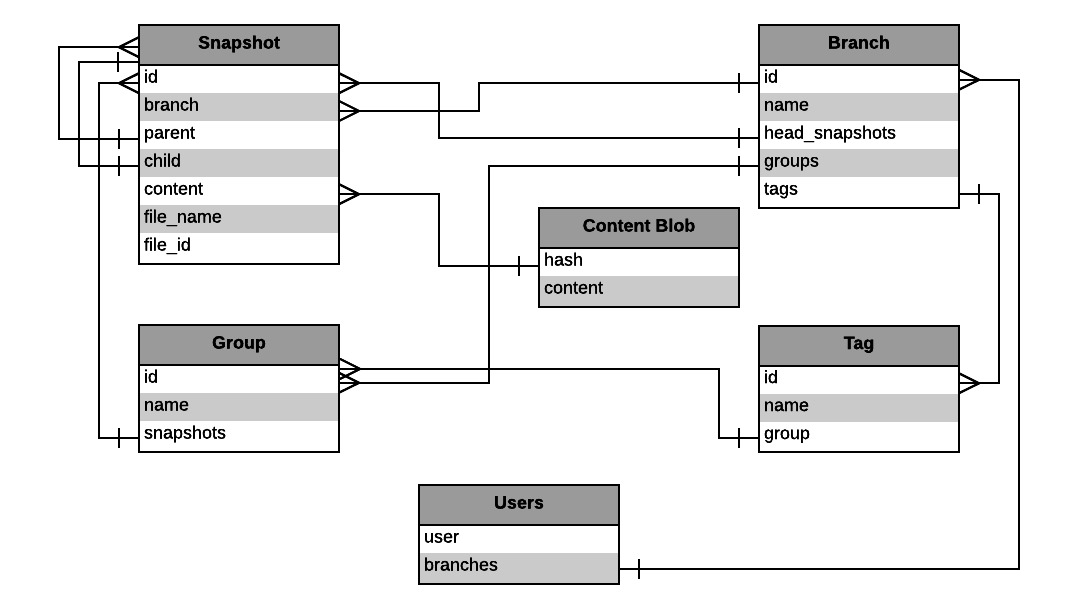
\includegraphics[max width= \linewidth]{DataModelServer}
\caption{Snapstore server data model.}
\label{arm:fig1}
\end{figure}

The user model on the server is a mapping of users to branches to which they have access. When a user shared a branch with another user, that branch is added to this mapping for that user. The server uses this mapping to share data with the appropriate users.

\section{User Interface}

**Pictures will go in here when the UI is done.**

\section{Keeping Data in Sync}

In Snapstore, users can work on a shared branch. As described in section 2.2.3, a shared branch is a line of development where a change from one user is propagated to all other users who are collaborators on that branch, keeping all of their Snapstore folders consistent.

However, this workflow can be difficult to maintain. Multiple users can be making edits at the same time, increasing concurrency issues. If two snapshots are made at the same time, there needs to be a way to resolve the snapshot graph. Also, a user can go offline and create snapshots, while their shared snapshot graphs are being written to by other, online users. Snapstore should be able to handle their reintroduction to the network without destroying the snapshot graph.

It is also important to maintain the ordering of events created by a single user. If a user creates a snapshot and then creates a group with that snapshot it in, it is necessary to send those two events in order to the server. Otherwise, the server might, for example, try to create a group containing a snapshot that doesn't exist.

We take the approach that any data that reaches the upstream server and is confirmed should be regarded as fact; it should never be undone. With this invariant, we designed a protocol algorithm for this process, called Distributed Event Synchronization Queue (DESQ).

\begin{center}
\begin{algorithm}[h]
\caption{DESQ}\label{euclid}
\begin{algorithmic}[1]
\Procedure{Client-DESQ}{}
\State $\textit{events} \gets \text{collection of }\textit{Events}$
\State $\textit{socket} \gets \text{server socket connection}$
\While {\emph{events} not empty}
\State $socket\text{.send(}events(0)\text{)}$
\EndWhile
\Loop{ on \emph{socket}.response(\emph{response, message})}:
\State Save \emph{response}
\If {$message == \text{"Confirm" or "Duplicate"}$}
\State \emph{events}.remove(\emph{events}(0))
\EndIf
\If {$message == \text{"Reject"}$}
\State $events\text{(0).data.parent} = response\text{(-1)}$
\EndIf
\EndLoop
\EndProcedure
\end{algorithmic}
%%%%%%%%%%%%%%%%%%%
\begin{algorithmic}[1]
\Procedure{Server-DESQ}{}
\State $\textit{db} \gets \text{MongoDB}$
\State $\textit{socket} \gets \text{client socket connection}$
\Loop{ on \emph{socket}.receive(\emph{event})}:
\If {$\textit{event} \text{.data.id in } \textit{db}$}
\State return $socket\text{.send(}event, \text{"Duplicate")}$
\EndIf
\If {$\textit{event}\text{.type } != \text{snapshot}$}
\State $event\text{.confirmed} \gets \text{True}$
\State $socket\text{.send(}event, \text{"Confirm")}$
\State return $socket\text{.room.send(}event, \text{"New Event")}$
\Else
\If {$event\text{.data.parent is head snapshot}$}
\State $event\text{.confirmed} \gets \text{True}$
\State $socket\text{.send(}event, \text{"Confirm")}$
\State return $socket\text{.room.send(}event, \text{"New Event")}$
\Else
\State $conflictSnapshots \gets \text{All snapshots between }event\text{.parent and }head$
\State return $socket\text{.send(}conflictSnapshots\text{,"Reject")}$
\EndIf
\EndIf
\EndLoop
\EndProcedure
\end{algorithmic}
\end{algorithm}
\end{center}

Each client has their own ordering of events, or database operations, that are stored in a client queue until they are confirmed by the server. The DESQ algorithm seeks to reach eventual consistency between these queues so that every client on a shared branch has the same data.

DESQ begins when an inconsistency is detected in the system. This can happen in two ways. First, if there is an event in the client's event queue, the algorithm will try to get that event confirmed by the server and shared with all appropriate users. Second, if a client connects to the server and detects that changes have been made, it will pull in those changes. Note that this protocol can proceed only when a network connection between the server and client is open. If they are closed, the events are queued until the network is available.

%Confirm + Duplicate
This algorithm pushes these events one at a time to the server repository. Events are confirmed if they can be applied to the server without causing any conflicts in the data. On the client, when an event is confirmed, it is removed from the event queue. Events also have a unique ID, so duplicate events can be caught and handled the same way.

%Push
When a client sends an event to the server and it is confirmed, the event must be propagated to all other collaborators. The server will find all clients that have access to that event's branch and send it to them. Because this is a confirmed event coming from the server, the other clients can apply this event to their local repository without adding it to their event queue.

%Reject
Snapshots are the only type of event that can cause a conflict, due to their inclusion in an ordered snapshot graph. All clients with access to this snapshot graph must agree on its order. The server will reject a client's snapshot event if the snapshot's snapshot graphs on the server and client are inconsistent. The rejected snapshot returns to the client with snapshots that will fix the inconsistencies.

In Git terms, if there is a conflict, the snapshot graph rebases and Snapstore tries to push that snapshot again. The rebasing keeps the snapshot graph and the workflow for the branch linear. However, while Git creates new commits during a rebase, Snapstore uses existing snapshots.

This protocol allows the system to handle consecutive rejections. This can occur when other clients are sending snapshot events to the server while another client's event is being rejected.


